\documentclass[conference]{IEEEtran}
\IEEEoverridecommandlockouts
% The preceding line is only needed to identify funding in the first footnote. If that is unneeded, please comment it out.
\usepackage{cite}
\usepackage{amsmath,amssymb,amsfonts}
\usepackage{graphicx}
\usepackage{textcomp}
\usepackage{xcolor}
\usepackage{booktabs}
\usepackage{url}
\def\BibTeX{{\rm B\kern-.05em{\sc i\kern-.025em b}\kern-.08em
    T\kern-.1667em\lower.7ex\hbox{E}\kern-.125emX}}

% ---------------------------------------------------------------------
%  Review mode. \blindtrue hides the authors and every self-identifying
%  link (repository, archive DOI, registrations) for double-blind review;
%  \blindfalse prints them (single-blind review and camera-ready).
% ---------------------------------------------------------------------
\newif\ifblind
\blindfalse

\newcommand{\polyforge}{PolyForge}
\newcommand{\jcac}{JCAC}
\newcommand{\rec}[1]{\texttt{\small #1}}   % a test tag or record in the artifact
\raggedbottom   % no stretched vertical space when a column ends short

\begin{document}

\title{When Does Joint Autoscaling Pay? A Pre-Registered Simulation Study
of Replica, Cache, and Model-Tier Control for LLM Serving}

% ---------------------------------------------------------------------
%  Alternative titles, if the primary does not suit the venue:
%
%  When Do Per-Layer Autoscalers Compose? A Pre-Registered Simulation
%  Study of Joint Replica, Cache, and Model-Tier Control for LLM Serving
%
%  Rate-Limited Autoscalers Compose: A Pre-Registered Test of Joint
%  Replica, Cache, and Model-Tier Control for LLM Serving
% ---------------------------------------------------------------------

\ifblind
\author{\IEEEauthorblockN{Anonymous Author(s)}
\IEEEauthorblockA{\textit{Affiliation withheld for double-blind review}}}
\else
\author{\IEEEauthorblockN{Md.\ Mohaiminul Islam}
\IEEEauthorblockA{\textit{Dept.\ of Electronics \& Telecommunication Engineering} \\
\textit{Rajshahi University of Engineering \& Technology}\\
Rajshahi 6204, Bangladesh \\
ORCID: 0009-0003-3254-9532}
% TODO(author): add the corresponding e-mail address on the line above.
\and
\IEEEauthorblockN{Farzana Akter}
\IEEEauthorblockA{\textit{Dept.\ of Electronics \& Telecommunication Engineering} \\
\textit{Rajshahi University of Engineering \& Technology}\\
Rajshahi 6204, Bangladesh}
% TODO(author): confirm the author list, order and e-mail addresses.
}
\fi

\maketitle

\begin{abstract}
Multi-tenant LLM serving platforms steer each tenant with three separate
controllers: a replica autoscaler such as the Kubernetes Horizontal Pod
Autoscaler (HPA), a semantic response cache, and a model-tier router. Joint
controllers that set all three at once rest on the premise that per-layer
decisions do not compose. We tested that premise in simulation on
\polyforge{}, a Kubernetes-native control plane whose planner chooses
replicas, cache budget and tier for every tenant by receding-horizon
search, within a program of 57 pre-registered protocols. An initial
advantage of 27.5\% in the composite objective $J$ over HPA, and of
53--60\% over a layered stack of per-layer controllers, disappeared as
registered re-scorings removed comparator defects: an inference charge only
the baselines paid, a pinned cache, edge-of-grid tuning, and a price-blind
tier rule. The joint controller ties tuned HPA ($-0.9\%$; an exploratory
equivalence analysis excludes differences above 5\%) and does not beat a
layered stack that routes to the cheapest tier, which is better by 23\% on
unseen, non-periodic demand. Barred from shedding AI traffic, it loses to
HPA. Coordination itself is worth 1.6\% of $J$, and nothing in a campaign
that also prices answer quality. A pre-registered width experiment explains
why. When one interval may move a tenant by at most two replicas and one
cache level, joint and per-knob search pick different moves in at most
1.04\% of decisions and are equivalent on all three simulated plants. With
$\pm8$-replica steps the gain grows four- to fivefold, but only where AI
work loads the replicas, and those steps make the controller worse.
\end{abstract}

\begin{IEEEkeywords}
autoscaling, LLM serving, multi-tenancy, semantic caching, model routing,
model predictive control, pre-registration, negative results
\end{IEEEkeywords}

% =====================================================================
\section{Introduction}
% =====================================================================

A platform that serves LLM traffic for many tenants decides, every few
seconds and for every tenant, how many replicas to run, how much
semantic-cache memory to grant, and which model tier answers the cache
misses. In practice each decision belongs to a different controller. HPA
or KEDA (Kubernetes Event-driven Autoscaling) scales replicas on a
utilization or queue signal~\cite{k8shpa,keda}; a semantic cache such as
GPTCache answers repeated prompts~\cite{gptcache}; and a router or cascade
sends the remaining requests to a cheaper or stronger
model~\cite{frugalgpt,routellm}, served by an engine such as
vLLM~\cite{vllm}. The layers share capacity. AI requests consume replica
time, a cache hit removes a model call, and the tier sets how long each
miss occupies the replicas. It is therefore natural to expect that
per-layer decisions do not compose, and that one controller should set all
three knobs together.

Joint control of serving knobs is an active line of work. INFaaS selects
model variants together with VM- and model-level
autoscaling~\cite{infaas}; IPA chooses variant, replication and batch size
on Kubernetes~\cite{ipa}; Proteus scales accuracy with placement and query
assignment~\cite{proteus}; Cascadia co-designs cascade deployment and
routing~\cite{cascadia}; and Zhu et al.\ choose a cache policy and a model
selector together~\cite{zhu2023}. Such systems report gains over separately
configured or fixed alternatives. Yet comparisons of controllers are
sensitive to how well the baselines are tuned and
instrumented~\cite{chameleon,melis2018,henderson2018,zhang2026drl}. A joint
controller compared against an under-tuned or handicapped per-layer stack
looks better for reasons that have nothing to do with coordination.

Few evaluations isolate what coordination itself is worth. Doing so
requires holding the objective, forecaster, actuation limits, budgets and
cost model fixed, and changing only whether the knobs are searched
jointly. We built a joint controller and then used a pre-registered
evaluation to try to break our own result. \polyforge{} is a
Kubernetes-native control plane whose planner, \jcac{}, chooses replicas,
cache budget and model tier for every tenant by receding-horizon
block-coordinate search. Every test below was registered before it ran
unless marked exploratory or descriptive. Tests are scored per design
point with bootstrap intervals, corrected for multiplicity and read with
equivalence margins, so that ``no difference'' is a measured result
rather than a failed test.

The joint controller's advantage did not survive, and a final
pre-registered experiment shows why: under rate-limited actuation the
per-tenant joint problem is locally separable. This paper makes four
contributions:
\begin{itemize}
\item \textbf{An adjudication chain} (Sec.~\ref{sec:chain},
  Fig.~\ref{fig:chain}): the headline wins over HPA and over a layered
  stack are traced to named comparator defects and removed by separately
  registered re-scorings.
\item \textbf{A direct measurement of coordination}
  (Sec.~\ref{sec:remains}, Table~\ref{tab:post}): with all else fixed,
  joint search beats per-knob search by 1.6\% of $J$, by nothing in a
  quality-priced campaign, and loses on unseen demand.
\item \textbf{A mechanism, confirmed under pre-registration}
  (Sec.~\ref{sec:width}, Fig.~\ref{fig:width}): coordination grows with
  how far one interval may move, and only where the layers share capacity.
\item \textbf{Evaluation lessons and an open artifact}
  (Secs.~\ref{sec:method} and~\ref{sec:lessons}): a checklist for
  comparing joint controllers, and code, data and protocols that
  regenerate every number in this paper.
\end{itemize}

% =====================================================================
\section{Related Work}
\label{sec:related}
% =====================================================================

\textit{Joint control of serving knobs.} Clipper combined a prediction
cache with adaptive model selection~\cite{clipper}. INFaaS, IPA and
Proteus decide model variants together with resources~\cite{infaas,ipa,
proteus}; Cascadia optimizes cascade deployment and routing as one
problem~\cite{cascadia}; and Zhu et al.\ show that caching and model
selection should be chosen together~\cite{zhu2023}. Cheng and Nguyen
allocate model, GPUs, parallelism and routing offline as a mixed-integer
program~\cite{chengnguyen2026}; and AIBrix pairs an LLM autoscaler with a
cost- and SLO-aware GPU optimizer~\cite{aibrix}.
\polyforge{} differs in its triple of knobs (replicas, a semantic-cache
budget and a model tier per tenant, under per-tenant dollar budgets) and,
more importantly, in what it measures. We report the value of
coordination with everything else held fixed, not the gain of one system
over a separately configured one.

\textit{Coordination of independent controllers.} Uncoordinated power
managers have been shown to fight one another~\cite{nopowerstruggles};
independent autonomic managers can be coordinated through one shared
signal~\cite{kephart2007}; and independent per-service autoscalers
oscillate where a coordinated one does not~\cite{chamulteon}. Process
control has long asked when decentralized loops suffice, and Bristol's
relative gain array measures the interaction that decides
it~\cite{bristol1966}. Our result is a discrete analogue for autoscaling.
With bounded per-interval steps, per-layer search over a shared objective
found the joint move in our setting.

\textit{Evaluation methodology.} Autoscalers should be compared on a level
playing field~\cite{chameleon}. Careful re-evaluations have
overturned reported gains in language modeling~\cite{melis2018} and
shown how fragile reported results are in deep reinforcement
learning~\cite{henderson2018}. In autoscaling, a calibrated rule-based
scaler beat six deep RL methods on cost~\cite{zhang2026drl}, and a
pre-registered evaluation of learned orchestrators found most predicted
advantages absent~\cite{khilji2026}. We follow the same discipline:
pre-registration~\cite{nosek2018}, benchmarking rules for performance
results~\cite{hoefler2015}, Holm correction~\cite{holm1979} and
equivalence tests~\cite{lakens2017}.

% =====================================================================
\section{System and Evaluation Method}
\label{sec:method}
% =====================================================================

\subsection{\polyforge{} and the \jcac{} planner}
\label{sec:jcac}

\polyforge{} consists of a Go control plane and AI gateway (tenant
isolation, rate limits, a per-tenant semantic cache), a Python planner,
and a Kubernetes operator that applies plans under guardrails: replica
bounds, at most one cache level per step, per-tenant budget caps, and a
last-good-plan fallback. The deployed planner imports the simulator's
controller module; the solver configuration evaluated below (anchored
moves, convergent sweeps) is selected in the operator's Helm chart, where
both options are off by default.

Every 10\,s, \jcac{} chooses for each tenant $i$ a configuration
$x_i=(r_i,c_i,\tau_i)$ (replicas, cache level, model tier) from a lattice
anchored at the interval-start state: $\Delta r\in\{-2,\dots,2\}$, a move
of at most one cache level (0, 64, 128, 256, 512 or 1024\,MB), and
$\tau\in\{\text{none},\text{small},\text{mid},\text{large}\}$, where
``none'' makes no model call. That gives at most 60 candidates per tenant.
Over a six-step (60\,s) forecast horizon it minimizes
\begin{equation}
\label{eq:plan}
\begin{split}
\Phi(x)={}&\frac{\alpha}{c_0}\sum_i \mathrm{cost}_i
 +\beta\sum_i\log\bigl(1+\mathrm{exc}_i\bigr)\\
 &+\gamma'\bigl(1-\mathrm{Jain}(s)\bigr)
 +\lambda\sum_i \mathrm{sw}_i ,
\end{split}
\end{equation}
where $\mathrm{cost}_i$ is projected spend (replica time, cache memory and
tier price per cache miss) and $\mathrm{exc}_i$ is the traffic-weighted
relative overshoot of p95 latency over the tenant's service-level
objectives (SLOs). The violation $v_i\in[0,1]$ is the same overshoot
capped at 1 per request family, and $s_i=1-v_i$ enters Jain's
index~\cite{jain1984}. $\mathrm{sw}_i$ counts changed knobs, with
$\alpha=1$, $\beta=2$, $\gamma'=0.5$, $\lambda=0.05$ and $c_0=\$0.01$ per
tenant-step. (An interference penalty that is zero unless a tenant is
flagged as a noisy neighbor is omitted.) A per-tenant dollar budget is a
hard filter: a candidate over budget is never scored. A tenant is
\emph{shed} when its tier is ``none'', either because that lowers $\Phi$
or because no candidate is affordable; the outage is priced only through
violation.

The solver is block-coordinate descent over tenants: each tenant
best-responds exactly over its lattice with the others fixed, and sweeps
repeat until a full sweep changes no tenant. Moves must strictly improve.
With uniform fairness weights $\Phi$ is an exact
potential~\cite{monderer1996}, so the final plan is a best response for
every tenant. A 50-sweep safety cap was never reached where it was counted
(\rec{JOINTNESS}). The published two-sweep planner took a median 73\,ms per
cycle for 8 tenants on one laptop core (p95 97\,ms); the convergent solver
was not timed separately. Only the first action is applied before
re-planning.

\begin{figure*}[!t]
\centering
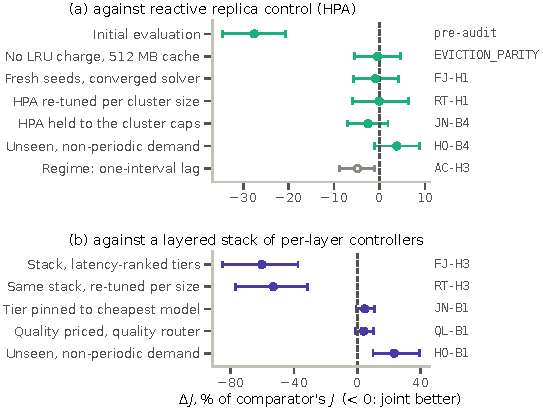
\includegraphics[width=\textwidth]{figures/fig_chain.pdf}
\caption{How the joint controller's advantage vanished. Each row is
\jcac{} minus comparator on $J$ at the design-point unit, as a percentage
of the comparator's $J$, with the 95\% bootstrap interval; negative means
\jcac{} is better. In (a) each step keeps the changes above it; tags name
the registered test, and the first two rows are exploratory re-analyses of
earlier matrices. The \rec{QL-B1} row compares $J_q$, which also prices
answer quality. The hollow row is a regime rather than a step: with
replicas one interval late, \jcac{} beats capped HPA.}
\label{fig:chain}
\end{figure*}

\subsection{Simulator, workloads and objective}
\label{sec:sim}

We call the simulated system the \emph{plant}. Demand is expressed in
work units: a replica serves 100 units/s and does the per-request work of
every call, so AI requests load the replicas (a chat request costs 20
units, an agent step 40) before calling a model. Models run outside the
plant: each tier has a price per request (\$0, \$$10^{-4}$, \$$10^{-3}$
and \$$10^{-2}$) and a base latency, and agent traffic needs a mid or
larger tier to avoid tool-loop retries. Batching, KV-cache memory, request
backlog and tier-switch lag are not modeled, and the planner plans with
the plant model it is scored on (Sec.~\ref{sec:threats}). A cache of $c$\,MB
hits a fraction $0.85\,c/(c+256)$ of a workload's cacheable share.

The main matrix crosses five workload classes (steady and bursty CRUD,
cacheable and uncacheable AI, agentic) with four eight-tenant mixes
(uniform, premium-heavy, best-effort-heavy, one dominant tenant) and three
cluster sizes (per-tenant replica caps of 6, 10 and 16). That gives 60
\emph{design points} of 120 steps each. The held-out campaign replaces the
workloads with two Markov-modulated bursty ones that no tuning slice or
earlier campaign had used (24 design points). The width experiment keeps
the four AI-carrying classes, including a bursty, cacheable, tier-mixed
joint-stress class (48). In every post-audit campaign each arm runs 5 reps
per design point on shared seeds, so all arms see identical demand; the
pre-audit matrices did not share seeds. Arms are scored on
\begin{equation}
\label{eq:J}
J=\overline{\mathrm{cost}}/c_0+2\,\bar v+0.5\,\bigl(1-\overline{\mathrm{Jain}}\bigr),
\end{equation}
the cost per scored tenant-step normalized by $c_0$, plus the mean
violation $\bar v$ and the mean unfairness. $J$ prices violation where
(\ref{eq:plan}) plans on log-excess. Planning on violation instead raises
$J$ by $0.0047$ $[-0.0025,+0.0121]$, an interval that includes zero
(\rec{JOINTNESS}, descriptive).

\subsection{Comparators}
\label{sec:comparators}

HPA and KEDA arms scale replicas on utilization and request rate, clamped
like \jcac{} to $\pm2$ replicas per interval, with a fixed cache and tier.
Their final versions are tuned on a separate slice over grids whose optima
are interior, re-tuned per cluster size, and held to the same cluster caps
as \jcac{}; Sec.~\ref{sec:chain} traces each step. Layered stacks run an
HPA rule, a cache policy and a tier rule independently, with four tier
rules: the registered one, which ranks tiers by latency and ignores price;
one that picks the cheapest tier expected to meet the latency target; a
pin to the cheapest model; and a quality-aware router. A static equal share
is the null controller. Only \jcac{} enforces the per-tenant budget and
only \jcac{} can shed; the comparators never shed and overrun the budget
on 3--4\% of tenant-steps (\rec{JOINTNESS}). Two ablations of \jcac{}
isolate coordination. They share its objective, forecast, budget filter
and lattice, and change only the knob search. The \emph{decoupled} arm
best-responds each knob with the other two held at the incumbent and then
combines the three winners, repairing only feasibility. The
\emph{knob-wise} arm moves one knob at a time to its best value and
repeats until no knob changes, never scoring a two-knob move.

\subsection{Statistics and pre-registration}
\label{sec:stats}

The unit of analysis is the design point, with reps averaged. A
directional claim PASSES only if a one-sided Wilcoxon signed-rank test
clears its Holm threshold within the campaign's registered family and the
95\% bootstrap interval of the mean paired difference (10{,}000 resamples)
lies on the registered side of zero. We say a comparison \emph{ties} or
shows no difference when that interval spans zero. Only an equivalence
reading (EQ: the 95\% interval inside the registered margin of
$\pm0.025$\,$J$, about 6\% of \jcac{}'s $J$ on the main matrix) bounds a
difference's size. Most campaigns also carry a non-inferiority guard on
SLO excess. Each protocol fixes arms, design, tests and predicted outcomes
and was committed and pushed before its first run. Two disclosed
exceptions, \rec{EVICTION\_PARITY} (Fig.~\ref{fig:chain}(a), second row)
and \rec{ORDER\_PERMUTATION}, were committed after their first runs. A
timing check compares every campaign's first run with its protocol's
commit; the pushes of the protocols written after the audit are also
recorded server-side by the CI runs they triggered. Test tags name the
campaign: FJ, RT, JN, AC, QL, HO, WD and SM stand for FAIR\_J, RETUNED,
JOINTNESS, ACTUATION, QUALITY, HELDOUT, WIDTH and STRUCTURAL\_MISMATCH.
Across all 57 protocols, 122 registered tests carry a $p$-value and 74
passed as registered; 57 of these also survive a Holm correction across
the whole program. The 81 gated records and 23 figures regenerate
byte-identically from the committed exports; 18 further records, such as
machine-dependent timings, are outside the gate with stated reasons.

% =====================================================================
\section{Results}
\label{sec:results}
% =====================================================================

\subsection{The adjudication chain}
\label{sec:chain}

Fig.~\ref{fig:chain}(a) follows the comparison with HPA. As first
reported, \jcac{} led by 27.5\% of HPA's $J$. Those comparators paid a
$1.4581\times$ surcharge on inference cost, modeling LRU cache eviction,
that \jcac{} did not, and ran a cache pinned at 128\,MB. Removing the
surcharge and sizing their cache like \jcac{}'s erased the lead
($-0.4\%$). With fresh shared seeds and the convergent solver the
difference is $-0.0037$ $[-0.0234,+0.0166]$, $-0.9\%$ (\rec{FJ-H1},
FAIL), and an exploratory equivalence analysis (90\% interval, two
one-sided tests) excludes any difference larger than 5.0\% of HPA's $J$.
The published HPA optimum had sat on a grid edge. Re-tuned per cluster
size over grids with interior optima, HPA ties ($-0.0001$
$[-0.0239,+0.0257]$, \rec{RT-H1}). This tie is a trade rather than an
identity: \jcac{} costs 19.3\% less but its mean violation is 60.1\%
higher, and every SLO guard in that campaign fails. Held to the same
cluster caps, HPA still ties (\rec{JN-B4}). On unseen bursty demand the
point estimate turns against \jcac{} ($+3.8\%$, interval spanning zero,
\rec{HO-B4}). Against KEDA without the surcharge, \jcac{} wins
(\rec{FJ-H2}, $-0.0305$) but not after re-tuning (\rec{RT-H2}, FAIL); held
to the cluster caps, re-tuned KEDA loses again (\rec{JN-B5}).

Fig.~\ref{fig:chain}(b) follows the layered stack. The registered stack
lost to \jcac{} by 60.4\% (\rec{FJ-H3}) and, re-tuned, by 53.1\%
(\rec{RT-H3}). Its tier rule ranks tiers by latency and ignores price,
which bought low violation at 3.7 times \jcac{}'s spend. Pin that stack's
tier to the cheapest model and the difference is $+0.0178$
$[-0.0032,+0.0416]$, no difference shown (\rec{JN-B1}). With a rule that
picks the cheapest tier expected to meet the latency target instead,
\jcac{} beats it by $0.3208$ (\rec{JN-B2}). In the quality-priced campaign
a quality-aware router shows no difference either (\rec{QL-B1}). On unseen
demand the cheapest-tier stack is better than \jcac{} by 23.3\%
($+0.0629$ $[+0.0268,+0.1065]$, \rec{HO-B1}). The 53--60\% win measured
one comparator's tier rule, not the value of joint control.

\begin{table*}[!t]
\caption{What survives the adjudications. \jcac{} minus comparator on
$J$: mean paired difference [95\% bootstrap CI] over design points (60
per column; 24 on unseen demand). Negative means \jcac{} is better.
B: \jcac{} better; T: no difference shown; W: \jcac{} worse; EQ: inside
the $\pm0.025$ equivalence margin. With instant actuation \jcac{} beats
only the static share and capped KEDA (and decoupled search, inside the
margin); with replicas one interval late it also beats capped HPA; on
unseen demand it beats nothing.}
\label{tab:post}
\centering
\footnotesize
\setlength{\tabcolsep}{4pt}
\begin{tabular}{@{}lccc@{}}
\toprule
Comparator & Instant actuation & Replicas one interval late & Unseen, non-periodic demand \\
\midrule
Decoupled search (same objective) & $-0.0066$ $[-0.0121,-0.0022]$ B, EQ & --- & $+0.0045$ $[+0.0020,+0.0073]$ W, EQ \\
Layered stack, cheapest tier & $+0.0178$ $[-0.0032,+0.0416]$ T & $+0.0069$ $[-0.0135,+0.0300]$ T & $+0.0629$ $[+0.0268,+0.1065]$ W \\
Static equal share & $-0.0235$ $[-0.0422,-0.0050]$ B & $-0.0227$ $[-0.0416,-0.0040]$ B & $-0.0109$ $[-0.0323,+0.0112]$ T \\
HPA, re-tuned, capped & $-0.0104$ $[-0.0290,+0.0076]$ T & $-0.0204$ $[-0.0371,-0.0045]$ B & $+0.0122$ $[-0.0035,+0.0284]$ T \\
KEDA, re-tuned, capped & $-0.0229$ $[-0.0438,-0.0022]$ B & $-0.0279$ $[-0.0474,-0.0089]$ B & $-0.0151$ $[-0.0377,+0.0073]$ T \\
\midrule
Registered tests & \rec{JN-C1}, \rec{JN-B1}, \rec{B3}--\rec{B5} & \rec{AC-H1}--\rec{H4} & \rec{HO-C1}, \rec{HO-B1}, \rec{B3}--\rec{B5} \\
\bottomrule
\end{tabular}
\end{table*}

\subsection{What remains of the joint controller's advantage}
\label{sec:remains}

Table~\ref{tab:post} collects the comparisons that survive the chain.
Coordination itself is small. With every other component fixed, joint
search lowers $J$ by $0.0066$ $[0.0022,0.0121]$ against decoupled search,
1.6\% of $J$, and by $0.0009$ against knob-wise search; both differences
lie inside the equivalence margin (\rec{JN-C1}, \rec{JN-C2}). The
quality-priced campaign adds twice the answer-quality loss to $J$, using a
quality index from published benchmark scores of three model
sizes~\cite{qwen25}, prices tiers at measured GPU cost and drops the budget
filter. There the difference is $+0.0012$ $[-0.0016,+0.0043]$
(\rec{QL-C1}, EQ). On unseen demand the decoupled search is better
(\rec{HO-C1}).

\jcac{}'s remaining wins come from three places (descriptive). The first
is cluster size. Against capped HPA it is better on the large cluster
($-0.0455$ $[-0.0720,-0.0192]$) and shows no difference on the small and
medium ones; on the small cluster the cheapest-tier stack beats it
($+0.0732$). The second is actuation lag. When replicas serve one interval
after they are added and grown caches start half-warm, it beats capped HPA
by 4.8\% and capped KEDA by 6.5\%, with both SLO guards passing
(\rec{AC-H3}, \rec{AC-H4}). The third is shedding: \jcac{} sheds AI
traffic on 7.2\% of tenant-steps. Held to never shedding, it is worse by
$0.0677$ $[0.0432,0.0945]$ and loses to capped HPA. Against most baselines
its SLO guard fails, because it buys its cost savings with more SLO
excess. On unseen demand, tested with instant actuation only, none of its
instant-actuation wins survives, and it sheds 11.3\% of tenant-steps.

\subsection{Why coordination buys little}
\label{sec:width}

\begin{figure}[!t]
\centering
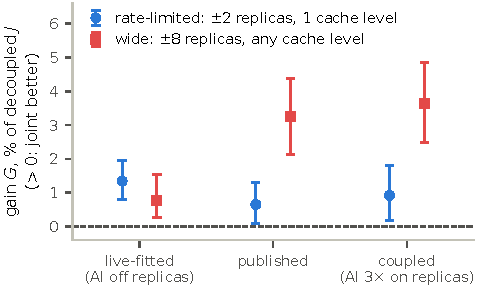
\includegraphics[width=\columnwidth]{figures/fig_width.pdf}
\caption{Coordination grows with step width only on plants where AI work
loads the replicas; on the rate-limited lattice it is small (0.7--1.3\%
of $J$) on every plant. Gain $G=J(\text{decoupled})-J(\text{joint})$, as
a percentage of the decoupled arm's $J$ ($>0$: joint better), with 95\%
bootstrap intervals (48 AI-carrying design points $\times$ 5 reps per
plant).}
\label{fig:width}
\end{figure}

Consider tenant $i$ at its incumbent and a candidate move
$\delta=(\delta_r,\delta_c,\delta_\tau)$. To second order the change in
$\Phi$ is $\sum_k g_k\delta_k+\frac12\sum_{k,l}H_{kl}\delta_k\delta_l$.
The decoupled search sees every first-order term and every diagonal term
but no cross term $H_{kl}\delta_k\delta_l$ with $k\neq l$. It therefore
recovers the joint move unless a cross term is large enough to reverse a
per-knob choice. Per-knob gains grow with $|\delta|$ and cross terms with
$|\delta|^2$, so the smaller the admissible step, the rarer a reversal.
Cache and tier always interact through the cost of a miss (tier price
times miss rate), which leaves a small gain at any width. Replica cross
terms exist only where AI work loads the replicas. This is a heuristic
sketch, not a proof, since the tier is categorical, and it makes two
testable predictions: coordination should grow once one step can be
large, and only where the layers share capacity.

\begin{table}[!t]
\caption{Width experiment: coordination gain $G$ on the rate-limited
($G_n$) and wide ($G_w$) lattices, their difference
$\mathrm{DiD}=G_w-G_n$ [95\% CI], and the joint arm's own $J_n-J_w$. The
gain grows with width on the published and coupled plants only, and the
wide lattice raises the joint arm's $J$ on every plant (48 AI-carrying
design points per plant; Table~\ref{tab:post}'s matrix also has CRUD
workloads).}
\label{tab:width}
\centering
\footnotesize
\setlength{\tabcolsep}{2.4pt}
\begin{tabular}{@{}lrrcr@{}}
\toprule
Plant & $G_n$ & $G_w$ & DiD [95\% CI] & $J_n-J_w$ \\
\midrule
Live-fitted & $+0.0033$ & $+0.0021$ & $-0.0012$ $[-0.0032,+0.0009]$ & $-0.0301$ \\
Published & $+0.0044$ & $+0.0231$ & $+0.0187$ $[+0.0082,+0.0287]$ & $-0.0152$ \\
Coupled   & $+0.0092$ & $+0.0407$ & $+0.0315$ $[+0.0161,+0.0472]$ & $-0.0859$ \\
\midrule
Tests & \multicolumn{2}{l}{H4: EQ, all} & H1, H2 PASS; H3 EQ & H5 PASS \\
\bottomrule
\end{tabular}
\end{table}

The width experiment tested both predictions on three plants. The
\emph{published} plant is the one used above. In the \emph{coupled} plant,
AI work loads the replicas three times as heavily and the mid and large
tiers cost two and four times the small tier's replica work. The
\emph{live-fitted} plant is fitted to measurements of the deployed system,
where a replica serves 1{,}123 units/s and AI requests never load the
replicas. On each plant, joint and decoupled search ran on the published
lattice and on a wide one ($\Delta r\in\{-8,\dots,8\}$, any cache level),
for 2{,}880 runs in all.

All five registered predictions held (Table~\ref{tab:width},
Fig.~\ref{fig:width}). On the rate-limited lattice the coordination gain
is small (0.7--1.3\% of the decoupled arm's $J$) and equivalent to zero on
every plant (\rec{WD-H4}), and the two searches choose different moves in
at most 1.04\% of best responses. On the wide lattice the gain grows by
$+0.0187$ on the published plant and $+0.0315$ on the coupled one
(\rec{WD-H1}, \rec{WD-H2}), and disagreement rises to 2.4\% and 3.9\%. On
the live-fitted plant it does not grow (\rec{WD-H3}, EQ; disagreement at
most 0.23\% at either width). Wide steps also make the joint controller
itself worse on every plant (\rec{WD-H5}): the regime in which
coordination pays is one this controller should not run in. The protocol
was written after exploratory probes on disjoint seeds, which it
discloses, so this is a confirmatory replication rather than a blind test.
Across the whole program, \rec{WD-H2} and \rec{WD-H5} on the coupled and
live-fitted plants survive Holm correction, \rec{WD-H1} survives only a
Benjamini--Yekutieli false-discovery-rate correction~\cite{by2001}, and
\rec{WD-H5} on the published plant only its registered family.

% =====================================================================
\section{Lessons}
\label{sec:lessons}
% =====================================================================

\textit{When to build a joint controller.} In our simulator, per-knob
search over a shared objective and forecast picked the joint move in at
least 98.96\% of decisions whenever per-interval steps were bounded. Joint
search earns its complexity only when one interval may move a tenant far
relative to its size \emph{and} the layers draw on a common resource.
Production autoscalers expose this bound. HPA's scaling policies cap how
many pods, or what percentage, one period may add or remove; by default a
deployment may double, or grow by four pods, every 15\,s, and scale-down
is damped by a 300\,s window~\cite{k8shpa}. At the tenant sizes we
simulate (6 to 16 replicas) that default scale-up is comparable to our
wide lattice, while the published lattice corresponds to a policy of two
pods per period. Bounding steps is therefore a configuration choice under
which, in our setting, per-layer autoscalers compose; in our simulator it
also lowered $J$ (\rec{WD-H5}).

\textit{How to evaluate one.} Every comparator defect we found favored the
joint controller. Exploratory re-analyses exposed them, and registered
re-scorings removed them. A comparison of joint against per-layer control
should (i)~charge every arm the same cost model, (ii)~give every arm the
same caps and actuation limits, (iii)~tune comparators per scale on grids
whose optima are interior, (iv)~include a static share and a layered stack
whose tier rule sees price, (v)~isolate coordination with a decoupled
ablation that keeps everything else fixed, (vi)~hold out demand that no
tuning saw, and (vii)~report equivalence margins and program-wide
corrections, not only failed superiority tests.

% =====================================================================
\section{Threats to Validity}
\label{sec:threats}
% =====================================================================

\textit{Substrate.} All comparisons ran in a simulator whose plant model
the planner also plans with, which favors \jcac{}. When the planner keeps
the published model while the plant follows the live-fitted one, the
layered stack beats it by $0.1052$ in $J$ (\rec{SM-H2}), so the simulator
flatters joint control rather than the reverse. One live case study on a
single GPU host (two reps, controller calibrated on the same plant) is in
the artifact; its five-seed replication was registered but not run, so we
make no live claim. \textit{Construct.} $J$'s weights are a choice. In an
exploratory re-scoring, the registered lateness weight (the weight of
violation in $J$) of 2 is exactly the crossover against re-tuned HPA: at
4, re-tuned HPA is better than \jcac{}, and at 8, re-tuned KEDA is too.
Shedding is priced only through violation. \textit{Internal.} The coupled
plant is a stress point chosen from a probe grid, not a measured system.
\textit{External.} Workloads are synthetic, periodic classes plus two
held-out Markov-modulated ones, with eight tenants per mix.

% =====================================================================
\section{Conclusion}
\label{sec:conclusion}
% =====================================================================

We set out to show that a joint replica, cache and tier controller beats
per-layer control for multi-tenant LLM serving, and found instead when it
does not. After the registered adjudications, the joint controller ties
tuned HPA, does not beat a cheapest-tier layered stack, and on unseen
demand beats no baseline. Coordination with everything else fixed is
worth 1.6\% of the objective, nothing in a quality-priced campaign, and it
reverses on unseen demand. The reason is local separability: with bounded
per-interval steps, per-knob search finds the joint move in all but at
most 1.04\% of decisions on every plant we tested, and coordination grows
only with wide steps on layers that share capacity, a regime that is worse
for this controller anyway. For practitioners, per-layer autoscalers that
share a forecast and an objective compose when their steps are bounded,
and a joint controller's gains can be read only after a comparator
checklist like ours. The next step is the registered five-seed live
replication, and a second is coordination under tier-switch lag and
backlog, which this simulator does not model.

\ifblind
\section*{Data Availability}
Code, simulator, protocols, raw run databases and the scripts that
regenerate every number and figure are available to reviewers in an
anonymized archive and will be published under a permanent DOI.
\else
\section*{Data Availability}
% TODO(author): before submission, publish the Zenodo version built on
% 2026-10-22 (eval/results/zenodo/polyforge-eval-artifact-2026-10-22.zip),
% which adds the HELDOUT and WIDTH run databases; the concept DOI below
% then resolves to it.
{\raggedright
Code and the run-level export of every campaign:
\url{https://github.com/mohaimin-8/polyforge}.\\
Raw run databases, protocols and the evaluation
artifact~\cite{polyforgezenodo}: \url{https://doi.org/10.5281/zenodo.22801195}.\\
Frozen copies of the first 48 protocols, made after those campaigns ran:
\url{https://doi.org/10.17605/OSF.IO/DYZKV}.\\
\texttt{python scripts/reproduce.py} regenerates every gated record and
figure; \texttt{research/paper-ieee/make\_figures.py} redraws the figures
of this paper from the same functions.\par}
\fi

% =====================================================================
%  REFERENCES
% =====================================================================

\begin{thebibliography}{00}

\bibitem{k8shpa}
Kubernetes Authors, ``Horizontal Pod Autoscaling,'' Kubernetes
documentation. Accessed: Oct.~22, 2026. [Online]. Available:
\url{https://kubernetes.io/docs/tasks/run-application/horizontal-pod-autoscale/}

\bibitem{keda}
KEDA Authors, ``KEDA: Kubernetes event-driven autoscaling.'' Accessed:
Oct.~22, 2026. [Online]. Available: \url{https://keda.sh}

\bibitem{gptcache}
F.~Bang, ``GPTCache: An open-source semantic cache for LLM applications
enabling faster answers and cost savings,'' in \textit{Proc. 3rd Workshop
Natural Lang. Process. Open Source Softw. (NLP-OSS)}, Singapore, 2023,
pp.~212--218.

\bibitem{frugalgpt}
L.~Chen, M.~Zaharia, and J.~Zou, ``FrugalGPT: How to use large language
models while reducing cost and improving performance,'' 2023,
\textit{arXiv:2305.05176}.

\bibitem{routellm}
I.~Ong \textit{et al.}, ``RouteLLM: Learning to route LLMs with preference
data,'' 2024, \textit{arXiv:2406.18665}.

\bibitem{vllm}
W.~Kwon \textit{et al.}, ``Efficient memory management for large language
model serving with PagedAttention,'' in \textit{Proc. 29th ACM Symp.
Operating Syst. Principles (SOSP)}, 2023, pp.~611--626.

\bibitem{infaas}
F.~Romero, Q.~Li, N.~J.~Yadwadkar, and C.~Kozyrakis, ``INFaaS: Automated
model-less inference serving,'' in \textit{Proc. USENIX Annu. Tech. Conf.
(ATC)}, 2021, pp.~397--411.

\bibitem{ipa}
S.~Ghafouri \textit{et al.}, ``IPA: Inference pipeline adaptation to
achieve high accuracy and cost-efficiency,'' \textit{J. Syst. Res.},
vol.~4, no.~1, 2024.

\bibitem{proteus}
S.~Ahmad, H.~Guan, B.~D.~Friedman, T.~Williams, R.~K.~Sitaraman, and
T.~Woo, ``Proteus: A high-throughput inference-serving system with accuracy
scaling,'' in \textit{Proc. 29th ACM Int. Conf. Architectural Support
Program. Lang. Operating Syst. (ASPLOS)}, 2024, pp.~318--334.

\bibitem{cascadia}
Y.~Jiang \textit{et al.}, ``Cascadia: An efficient cascade serving system
for large language models,'' 2025, \textit{arXiv:2506.04203}.

\bibitem{zhu2023}
B.~Zhu, Y.~Sheng, L.~Zheng, C.~Barrett, M.~I.~Jordan, and J.~Jiao,
``Towards optimal caching and model selection for large model inference,''
in \textit{Adv. Neural Inf. Process. Syst. (NeurIPS)}, vol.~36, 2023.

\bibitem{chameleon}
A.~Bauer, N.~Herbst, S.~Spinner, A.~Ali-Eldin, and S.~Kounev, ``Chameleon:
A hybrid, proactive auto-scaling mechanism on a level-playing field,''
\textit{IEEE Trans. Parallel Distrib. Syst.}, vol.~30, no.~4,
pp.~800--813, 2019.

\bibitem{melis2018}
G.~Melis, C.~Dyer, and P.~Blunsom, ``On the state of the art of evaluation
in neural language models,'' in \textit{Proc. Int. Conf. Learn.
Represent. (ICLR)}, 2018.

\bibitem{henderson2018}
P.~Henderson, R.~Islam, P.~Bachman, J.~Pineau, D.~Precup, and D.~Meger,
``Deep reinforcement learning that matters,'' in \textit{Proc. AAAI Conf.
Artif. Intell.}, vol.~32, no.~1, 2018.

\bibitem{zhang2026drl}
G.~Zhang, C.~Sun, K.~Zhao, X.~Chu, S.~Sarkani, and J.~Fossaceca, ``When
does deep RL beat calibrated baselines? A benchmark study on adaptive
resource control,'' 2026, \textit{arXiv:2605.26418}.

\bibitem{clipper}
D.~Crankshaw, X.~Wang, G.~Zhou, M.~J.~Franklin, J.~E.~Gonzalez, and
I.~Stoica, ``Clipper: A low-latency online prediction serving system,'' in
\textit{Proc. 14th USENIX Symp. Networked Syst. Des. Implement. (NSDI)},
2017, pp.~613--627.

\bibitem{chengnguyen2026}
J.~Cheng and D.~T.~Nguyen, ``Scalable joint resource allocation for
SLO-constrained LLM inference in heterogeneous GPU clouds,'' 2026,
\textit{arXiv:2604.07472}.

\bibitem{aibrix}
The AIBrix Team, ``AIBrix: Towards scalable, cost-effective large language
model inference infrastructure,'' 2025, \textit{arXiv:2504.03648}.

\bibitem{nopowerstruggles}
R.~Raghavendra, P.~Ranganathan, V.~Talwar, Z.~Wang, and X.~Zhu, ``No
`power' struggles: Coordinated multi-level power management for the data
center,'' in \textit{Proc. 13th Int. Conf. Architectural Support Program.
Lang. Operating Syst. (ASPLOS)}, 2008, pp.~48--59.

\bibitem{kephart2007}
J.~O.~Kephart, H.~Chan, R.~Das, D.~W.~Levine, G.~Tesauro, F.~Rawson, and
C.~Lefurgy, ``Coordinating multiple autonomic managers to achieve
specified power-performance tradeoffs,'' in \textit{Proc. 4th Int. Conf.
Autonomic Comput. (ICAC)}, 2007.

\bibitem{chamulteon}
A.~Bauer, V.~Lesch, L.~Versluis, A.~Ilyushkin, N.~Herbst, and S.~Kounev,
``Chamulteon: Coordinated auto-scaling of micro-services,'' in
\textit{Proc. IEEE 39th Int. Conf. Distrib. Comput. Syst. (ICDCS)}, 2019,
pp.~2015--2025.

\bibitem{bristol1966}
E.~H.~Bristol, ``On a new measure of interaction for multivariable process
control,'' \textit{IEEE Trans. Autom. Control}, vol.~11, no.~1,
pp.~133--134, 1966.

\bibitem{khilji2026}
S.~I.~Khilji, A.~Furutanpey, and S.~Dustdar, ``Incentives and evidence in
learned service orchestration,'' in \textit{Proc. IEEE Int. Congr.
Intell. Service-Oriented Syst. Eng. (CISOSE)}, 2026, to appear,
\textit{arXiv:2606.16555}.

\bibitem{nosek2018}
B.~A.~Nosek, C.~R.~Ebersole, A.~C.~DeHaven, and D.~T.~Mellor, ``The
preregistration revolution,'' \textit{Proc. Nat. Acad. Sci.}, vol.~115,
no.~11, pp.~2600--2606, 2018.

\bibitem{hoefler2015}
T.~Hoefler and R.~Belli, ``Scientific benchmarking of parallel computing
systems: Twelve ways to tell the masses when reporting performance
results,'' in \textit{Proc. Int. Conf. High Perform. Comput., Netw.,
Storage Anal. (SC)}, 2015.

\bibitem{holm1979}
S.~Holm, ``A simple sequentially rejective multiple test procedure,''
\textit{Scand. J. Statist.}, vol.~6, no.~2, pp.~65--70, 1979.

\bibitem{lakens2017}
D.~Lakens, ``Equivalence tests: A practical primer for $t$ tests,
correlations, and meta-analyses,'' \textit{Social Psychol. Personality
Sci.}, vol.~8, no.~4, pp.~355--362, 2017.

\bibitem{jain1984}
R.~Jain, D.-M.~Chiu, and W.~R.~Hawe, ``A quantitative measure of fairness
and discrimination for resource allocation in shared computer systems,''
Digital Equipment Corp., Tech. Rep. DEC-TR-301, 1984.

\bibitem{monderer1996}
D.~Monderer and L.~S.~Shapley, ``Potential games,'' \textit{Games Econ.
Behav.}, vol.~14, no.~1, pp.~124--143, 1996.

\bibitem{qwen25}
Qwen Team, ``Qwen2.5 technical report,'' 2024, \textit{arXiv:2412.15115}.

\bibitem{by2001}
Y.~Benjamini and D.~Yekutieli, ``The control of the false discovery rate
in multiple testing under dependency,'' \textit{Ann. Statist.}, vol.~29,
no.~4, pp.~1165--1188, 2001.

\ifblind\else
\bibitem{polyforgezenodo}
M.~M.~Islam, ``PolyForge evaluation artifact: Pre-registered
controller-comparison campaigns,'' Zenodo, 2026, doi:
10.5281/zenodo.22801195.
\fi

\end{thebibliography}

\end{document}
